\documentclass[10pt]{article}

\usepackage[a4paper, total={6.5in, 8in}]{geometry}
\usepackage{amssymb, amsmath, amsthm, graphicx, setspace, ctable, enumerate, appendix, ccaption, lineno, subcaption}
\usepackage[utf8]{inputenc}

\PassOptionsToPackage{%
    %backend=biber, %instead of bibtex
	backend=bibtex8,bibencoding=ascii,%
	language=auto,%
	%style=numeric-comp,%
    style=authoryear-comp, % Author 1999, 2010
    bibstyle=authoryear,dashed=false, % dashed: substitute rep. author with ---
    sorting=nyt, % name, year, title
    maxbibnames=10, % default: 3, et al.
    %backref=true,%
    natbib=true % natbib compatibility mode (\citep and \citet still work)
}{biblatex}
\usepackage{biblatex}

\newcommand{\thead}[1]{\textsc{#1}}
\newcommand{\theadr}[1]{\textsc{#1}}
\newcommand{\theadl}[1]{\textsc{#1}}
\newcommand{\ie}{i.\,e. }
\newcommand{\Ie}{I.\,e. }
\newcommand{\eg}{e.\,g. }
\newcommand{\Eg}{E.\,g. }
\newcommand{\super}[1]{\textsuperscript{#1}}
%\newcommand{\super}[1]{\tiny #1}


\addbibresource{beast2.bib}
%\addbibresource{Ebola.bib}
%\addbibresource{IDD.bib}

\doublespacing
\linenumbers

\begin{document}

	\thispagestyle{plain}
	\title{EBOV analysis example for BEAST 2.5}  
	\author{Louis du Plessis}
	\date{\today}
	\maketitle

	
	%\clearpage
	\begin{abstract}
		Phylodynamics example for BEAST 2.5 paper using data from the West African Ebola dataset. The example uses a sampled-ancestor birth-death skyline to infer population dynamics. This can also double as a bModelTest example.
	\end{abstract}

	\tableofcontents

	\clearpage
	
%\section*{bdsky results}
\section{Tree models for unstructured populations}


\begin{figure}[!ht]
	\includegraphics{figures/{EBOV-SUBBIG.BDSKYSA.BMT.relaxedclock.R20.SM.combined2}.pdf}
	\caption{Birth-death skyline (bdsky) analysis of the 2013--2016 West African Ebola virus disease epidemic.  
\textbf{(a)} The maximum clade credibility tree of the 811 sequences used in the analysis. 
\textbf{(b)} The median posterior estimate of the estimated effective reproductive number ($R_e$) over time is shown in orange, with the 95\% highest posterior density (HPD) interval in orange shading. The red dotted line indicates the epidemic threshold ($R_e = 1$). If $R_e$ is below this threshold the epidemic has reached a turning point and is no longer spreading. 
The posterior distribution of the origin time of the epidemic ($t_0$) is shown in green. 
The number of laboratory-confirmed cases per epiweek is shown in blue. Red arrows indicate weeks with fewer than 10 confirmed cases. The dotted line at A indicates the onset of symptoms in the suspected index case \citep{WHO2016NEJM}. The dotted lines at B and C indicate the dates at which the WHO declared an Ebola virus disease outbreak in Guinea and a Public Health Emergency of International Concern (PHEIC), respectively. The dotted line at D indicates the first time any of the three countries with intense transmission (Liberia) was declared Ebola free following 42 days without any new infections being reported (new cases were subsequently detected in Liberia in June 2015).
\textbf{(c)} The median posterior estimate of the monthly sampling proportion is shown in purple, with the 95\% HPD interval in purple shading.
The red dashed line indicates the number of sampled sequences in the dataset, divided by the number of laboratory-confirmed cases, for each month in the analysis. This serves as an empirical estimate of the true sampling proportion. 	
The posterior distributions and medians (dashed lines) of the infected period and the mean clock rate (truncated at the 95\% HPD limits) are shown in panels \textbf{(d)} and \textbf{(e)}.}
	\label{fig:ebov_bdsky}	
\end{figure}

\clearpage 

%\emph{Insert at the end of the paragraph ending on line 206 (bdsky)}


\noindent
In epidemiological investigations the birth-death model can be reparameterised by setting the rate of becoming noninfectious, $\delta = \mu + \psi r$ (the total rate at which lineages are removed), the effective reproductive number, $R_e = \lambda / \delta$, and the sampling proportion $p = \psi / \delta$ (the proportion of removed lineages that are sampled). 
Figure~\ref{fig:ebov_bdsky} shows the posterior estimates from a bdsky analysis of the 2013--2016 West African Ebola epidemic. Estimates are based on the coding regions of 811 sequences sampled through October 24, 2015, representing more than 2.5\% of known cases. 
There is evidence that hospital-based transmission and unsafe burials contributed infections to the epidemic \citep{Whitty2014Nature}, thus the sampled ancestor package was used to account for some percentage of patients continuing to transmit the virus after being sampled (by allowing $r$ to be less than 1). 
$R_e$ was allowed to change over 20 time intervals, equally-spaced between the origin of the epidemic ($t_0$) and the time of the most recent sample, while the the sampling proportion was estimated for every month from March 2014 onwards (when an Ebola virus disease outbreak was declared and the first samples collected). 
The estimated origin time of the epidemic coincides with the onset of symptoms in the suspected index case on December 26, 2013 \citep{WHO2016NEJM}.
Estimates of $R_e$ are consistent with WHO estimates \citep{WHO2015NEJM}, based on surveillance data alone, but with greater uncertainty. 
For the majority of the period between mid-May and October 2014 $R_e$ is estimated to be above 1, consistent with the observation that September 2014 was the turning point of the epidemic and that case incidence stopped growing in October \citep{WHO2015NEJM}. 
After peak incidence was reached during the last week of September 2014, $R_e$ estimates drop below 1 during October and November 2014 and then fluctuates around 1 during 2015 as transmissions persisted in some areas, due to a combination of unwillingness to seek medical care, unsafe burials and imperfect quarantine measures \citep{WHO2016NEJM}. % as transmission chains continued to emerge. 
$R_e$ estimates before May 2014 and after August 2015 have a large amount of uncertainty attached to them, due to the small amount of sequences sampled during these time periods.
Trends in sampling proportion estimates follow empirical estimates based on the number of confirmed cases, however the sampling proportion is overestimated during the period of intense transmission, which suggests the existence of transmission chains not represented in the sequence dataset. 
In the final two months of the study period the sampling proportion is underestimated, which may indicate ongoing cryptic transmission during this period, but may also be indicative of a model bias resulting from the remaining transmission chains at this time being highly isolated from each other, which is not taken into account by the model. 


% Although not done here, it is possible to account for the incubation time of an epidemic using the structured models discussed in the next section.


\clearpage

\section{Substitution models}


\begin{figure}[!h]
\centering
	\includegraphics[width=\textwidth]{figures/{EBOV-SUBBIG.BDSKYSA.BMT.relaxedclock.R20.SM.bModelAnalyser}.png}
	\caption{Posterior distribution of substitution models from an analysis of the 2013--2016 West African Ebola virus epidemic. Each circle represents a substitution model indicated by a six digit number corresponding to the six rates of reversible substitution models. In alphabetical order, these are
A$\to$C, A$\to$G, A$\to$T, C$\to$G, C$\to$T, and G$\to$T, which can be shared in groups.
The six digit numbers indicate these groupings, for example 121121 indicates the HKY model, which has shared rates for transitions and shared rates for transversions. 
Here, only models are considered that are reversible and do not share transition and transversion rates (with the exception of the Jukes Cantor model).
Other substitution model sets are available.
Links between substitution models indicate possible jumps during the MCMC chain from simpler (tail of arrow) to more complex (head of arrow) models and back.
There is no single preferred substitution model for this dataset, as the posterior probably is spread over a number of alternative substitution models.
Blue circles indicate the 13 models contained in the 95\% credible set, red are outside, and models without circles have neglegible support. 
In addition, the analysis indicated 100\% posterior probability for gamma-distributed rate heterogeneity across sites and unequal base frequencies.}
	\label{fig:ebov_bmt}	
\end{figure}

\clearpage

%\emph{Insert into substitution models section if it is included}

Figure~\ref{fig:ebov_bmt} shows the posterior distribution resulting from a bModelTest analysis of substitution models for 14,517 nucleotides from the coding regions of 811 EBOV sequences sampled during the 2013--2016 West African Ebola virus epidemic. 
Each circle represents a substitution model indicated by a six digit number corresponding to the six rates of reversible substitution models (see Figure~\ref{fig:ebov_bmt} caption for more details). 








	\clearpage
	\appendix
	\renewcommand{\thefigure}{S\arabic{figure}}
	\renewcommand{\thetable}{S\arabic{table}}	
	\setcounter{page}{1}
	\setcounter{figure}{0}
	\section{Materials and Methods}

\subsection{Sequencing and surveillance data}

	I downloaded 1,610 EBOV sequences, sampled between 17 March 2014 and 24 October 2015, used in the analyses presented in \citet{Dudas2017Nature}\footnote{\url{https://github.com/ebov/space-time.git}, downloaded on 8 August 2018.}.
	%I extracted the coding regions of the sequences and removed all sites with more than 95\% unknown bases (sites where 1,530 or more sequences have an unknown nucleotide). This resulted in an alignment of 14,517bp. 
	% Actually no sites were removed from CDS, only from IG... 
	I extracted the coding regions of the sequences, resulting in an alignment of 14,517 bp. Since no sites in the alignment contained more than 419 unknown bases (26\%), no sites were excluded from the alignment. 
	I further subsampled the dataset to 811 sequences (approximately 50\%). Subsampling was stratified by month to maintain the approximate sampling proportion over time (\ie within each month 50\% of sampled sequences were removed at random). In order to prevent a loss of phylogenetic signal, all sequences from months where less than 5 sequences were sampled were included in the final dataset. The weekly and monthly numbers of sampled sequences in the complete and subsampled datasets are shown in Figure~\ref{fig:seqdata_weekly} and~\ref{fig:seqdata_monthly}. The geographic distribution of sequences in the complete and subsampled datasets are shown in Figure~\ref{fig:seqdata_complete_geo} and~\ref{fig:seqdata_special-subbig_geo}.

	I downloaded weekly probable and confirmed numbers of newly reported cases for Guinea, Liberia and Sierra Leone from the WHO website\footnote{\url{http://apps.who.int/gho/data/node.ebola-sitrep}, downloaded on 10 June 2016.}. This included reported cases up to the week starting on 8 May 2016. 
	In weeks where data are available from the patient database and WHO situation reports I use the maximum of the two counts. 
	In all analyses I use only the number of laboratory confirmed cases.

	\begin{figure}[!p]
		\begin{subfigure}[b]{\textwidth}
			\centering
			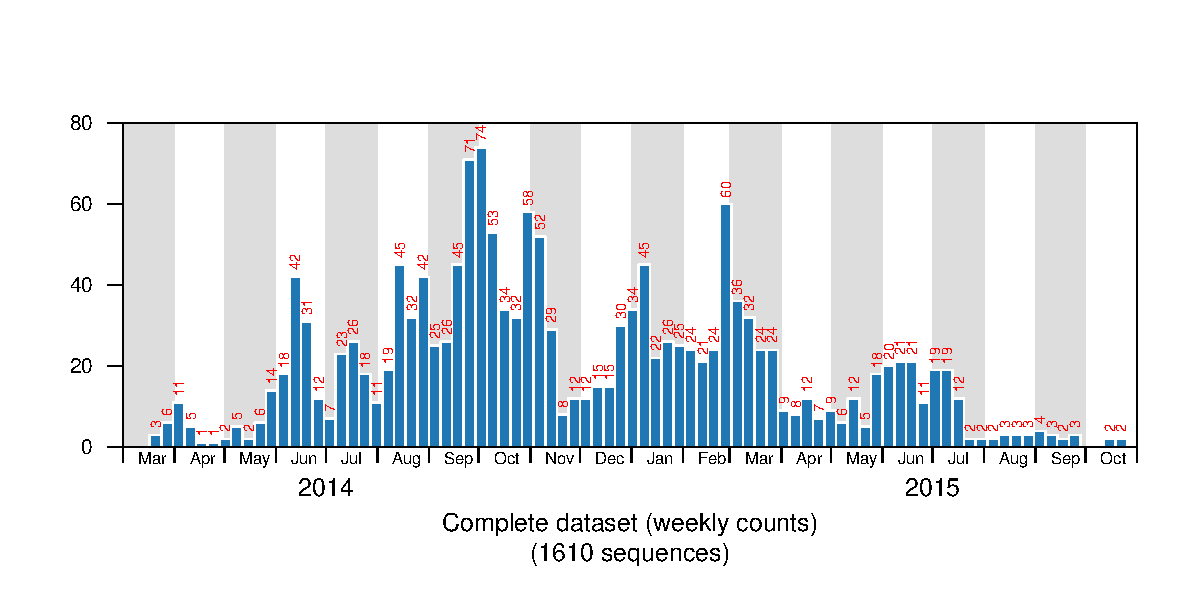
\includegraphics[width=\columnwidth]{figures/complete-date-1}
			%\subcaption{Complete dataset}			
		\end{subfigure}		
		\begin{subfigure}[b]{\textwidth}
			\centering
			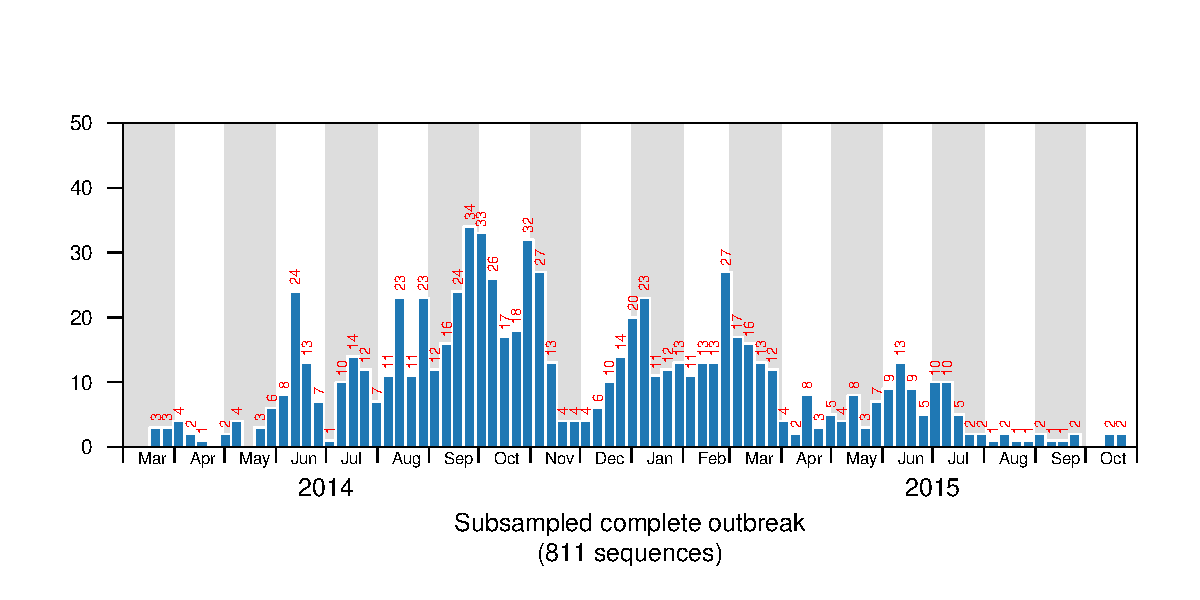
\includegraphics[width=\columnwidth]{figures/special-subbig-date-1}
			%\subcaption{Subsampled dataset}			
		\end{subfigure}
		\caption{Weekly numbers of sampled sequences in the complete and subsampled datasets.}
		\label{fig:seqdata_weekly}
	\end{figure}

	\begin{figure}[!p]
		\begin{subfigure}[b]{\textwidth}
			\centering
			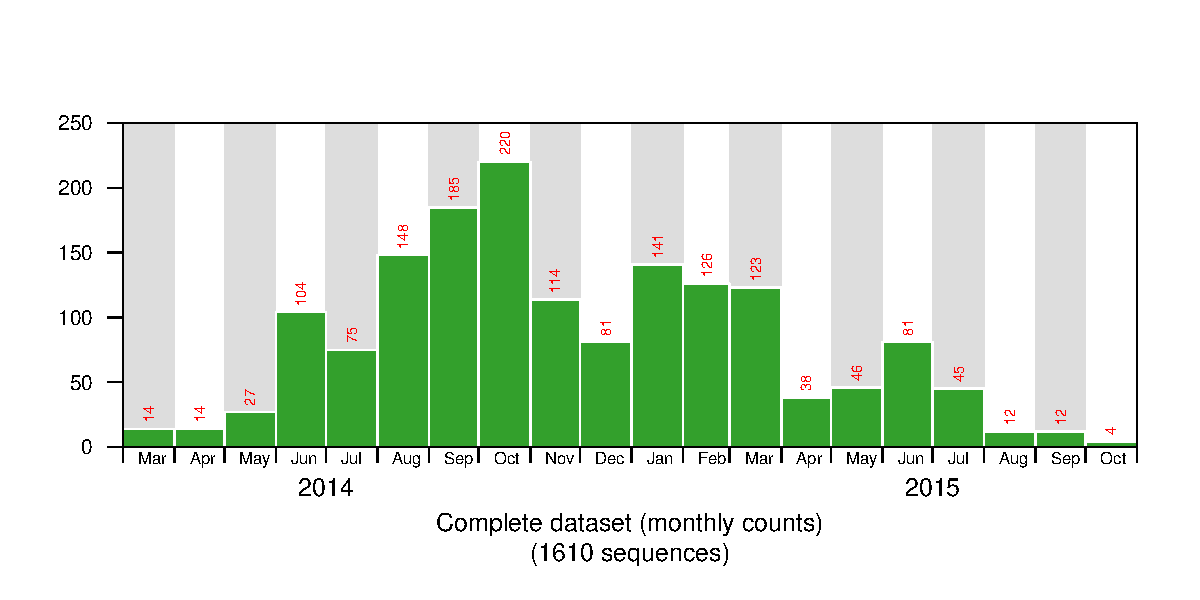
\includegraphics[width=\columnwidth]{figures/complete-date-2}
			%\subcaption{Complete dataset}			
		\end{subfigure}		
		\begin{subfigure}[b]{\textwidth}
			\centering
			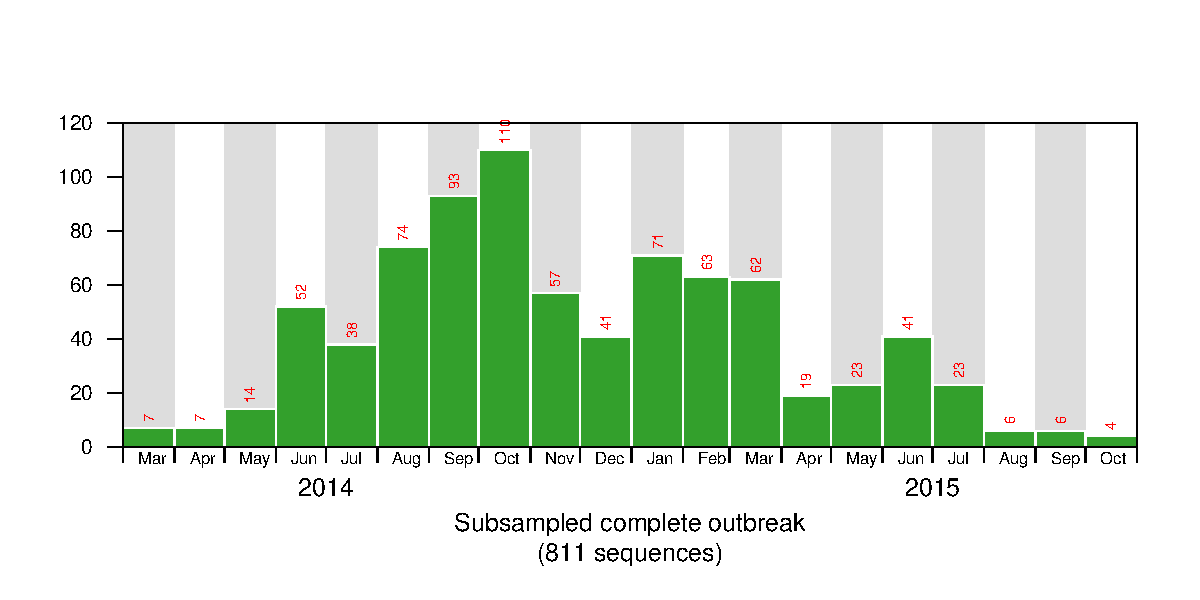
\includegraphics[width=\columnwidth]{figures/special-subbig-date-2}
			%\subcaption{Subsampled dataset}			
		\end{subfigure}
		\caption{Monthly numbers of sampled sequences in the complete and subsampled datasets.}
		\label{fig:seqdata_monthly}
	\end{figure}


	\begin{figure}[!p]
		\begin{subfigure}[b]{0.45\textwidth}
			\centering
			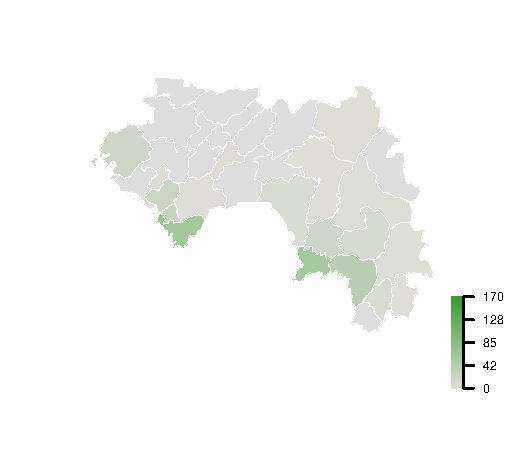
\includegraphics[width=\columnwidth]{figures/complete-geo-1}
			\subcaption{Guinea (GIN)}			
		\end{subfigure}		
		\hfill
		\begin{subfigure}[b]{0.45\textwidth}
			\centering
			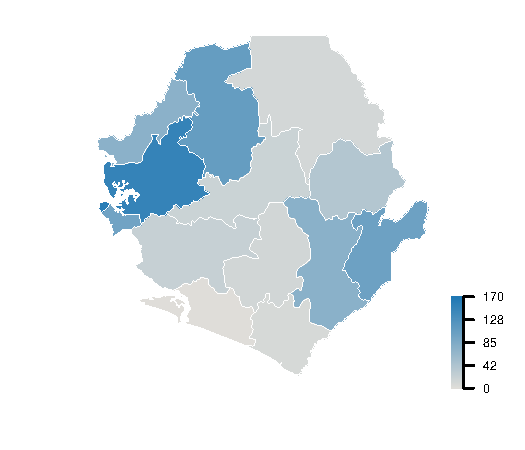
\includegraphics[width=\columnwidth]{figures/complete-geo-2}
			\subcaption{Sierra Leone (SLE)}			
		\end{subfigure}		
		\\
		\begin{subfigure}[b]{0.45\textwidth}
			\centering
			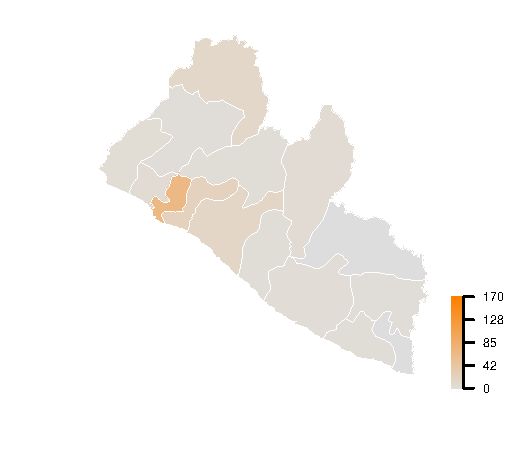
\includegraphics[width=\columnwidth]{figures/complete-geo-3}
			\subcaption{Liberia (LBR)}			
		\end{subfigure}		
		\hfill
		\begin{subfigure}[b]{0.45\textwidth}
			\centering
			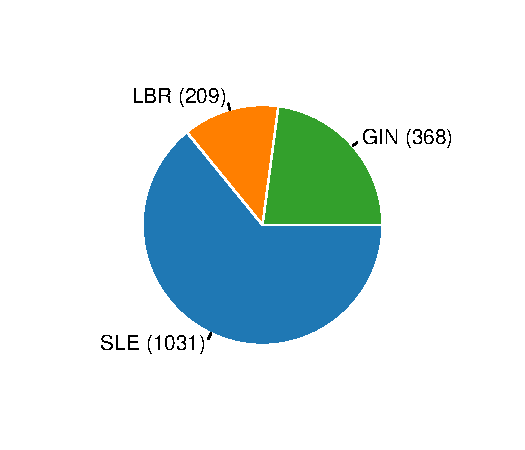
\includegraphics[width=\columnwidth]{figures/complete-geo-4}
			%\subcaption{Complete dataset}			
		\end{subfigure}		
		\caption{Geographic distribution of samples in the complete dataset.}
		\label{fig:seqdata_complete_geo}
	\end{figure}


	\begin{figure}[!p]
		\begin{subfigure}[b]{0.45\textwidth}
			\centering
			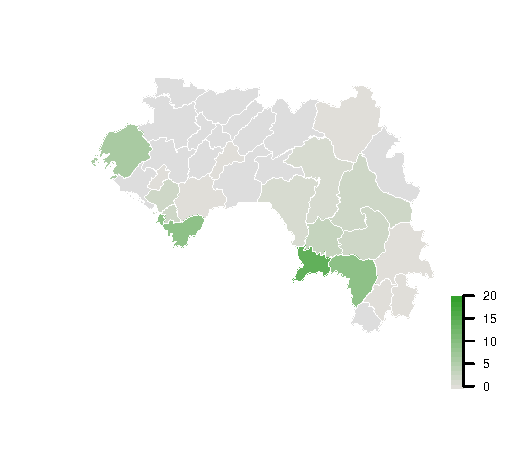
\includegraphics[width=\columnwidth]{figures/special-subbig-geo-1}
			\subcaption{Guinea (GIN)}			
		\end{subfigure}		
		\hfill
		\begin{subfigure}[b]{0.45\textwidth}
			\centering
			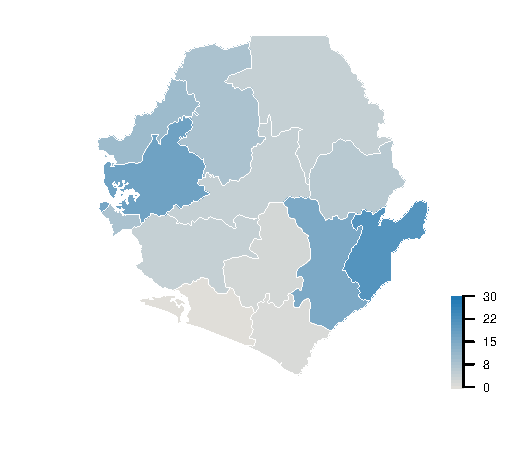
\includegraphics[width=\columnwidth]{figures/special-subbig-geo-2}
			\subcaption{Sierra Leone (SLE)}			
		\end{subfigure}		
		\\
		\begin{subfigure}[b]{0.45\textwidth}
			\centering
			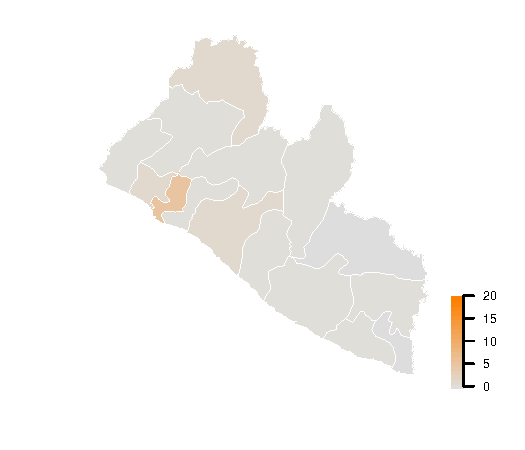
\includegraphics[width=\columnwidth]{figures/special-subbig-geo-3}
			\subcaption{Liberia (LBR)}			
		\end{subfigure}		
		\hfill
		\begin{subfigure}[b]{0.45\textwidth}
			\centering
			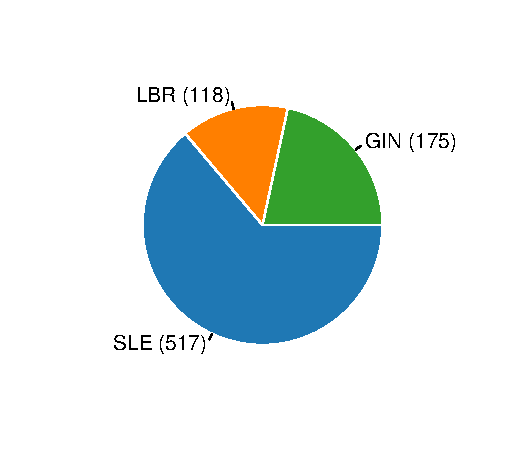
\includegraphics[width=\columnwidth]{figures/special-subbig-geo-4}
			%\subcaption{Complete dataset}			
		\end{subfigure}		
		\caption{Geographic distribution of samples in the subsampled dataset.}
		\label{fig:seqdata_special-subbig_geo}
	\end{figure}


\subsection{Phylodynamic analylses}

	The serially sampled birth-death skyline model \citep{stadler2013birth} was used as a tree-prior in the analyses. 
	A lognormal prior distribution with mean 0 and standard deviation 1.25 was placed on $R_e$, which was allowed to vary over 20 time intervals, equally spaced between the origin and the time of the most recent sample (October 24, 2015). 
	The sampling proportion was estimated for independently for every month between March 2014 and October 2015. A Beta-distributed prior with $\alpha = 2$ and $\beta = 10$ was placed on the sampling proportion for each month. Before March 2014 the sampling proportion was set to 0, since no sampling effort was made before this time.
	A normally-distributed prior with mean at January 1, 2014 and standard deviation of $~1.5$ months was placed on the origin parameter, which was further bounded to be after December 1, 2013. 
	A Beta-distributed prior with $\alpha = 5$ and $\beta = 2$ was placed on $r$ (the removal probability) and the sampled ancestor package \citep{gavryushkina2014bayesian} was used to allow sampled ancestors in the estimated tree. 
	The bModelTest \citep{bouckaert2017bmodeltest} package was used to perform Bayesian model averaging across all time-reversible substitution models with a transition/transversion ratio split, while simultaneously estimating support for gamma-distributed rate heterogeneity across sites and unequal base frequencies. 
	An uncorrelated lognormal relaxed clock model \citep{drummond2006} was used to estimate the substitution rate. A lognormal prior with mean $1.2 \times 10^{-3}$ s/s/y (in real space) and standard deviation 0.05 s/s/y was placed on the mean molecular clock rate parameter. 

	All analyses were performed in BEAST v2.5.0 \citep{bouckaert2014beast}. 
	I computed 8 independent MCMC chains of 100 million steps and sampled parameters and trees every 20,000 steps. 
	Tracer v1.7.1 \citep{Rambaut2018Tracer} was used to check convergence and Logcombiner v2.5.0 was used to combine and subsample chains, removing 25\% as burn-in and resampling parameters every 100,000 steps. 
	Treeannotator v2.5.0 was used to produce the maximum clade credibility tree, from the combined and subsampled posterior tree distribution, using median heights. 

	Figures were produced using the R software platform using in-house scripts and the R-package bdskytools (available at \url{https://github.com/laduplessis/bdskytools}) and ggtree \citep{Yu2017}. 
	Further details are available at \url{https://github.com/laduplessis/Beast2Example}.


\section{Comparison to other studies}

\subsubsection*{Reproductive number estimates}

	Estimates of $R_e$ are always below 3 and fall between 1 and 2 for the majority of the growth phase of the epidemic. This is consistent with nearly all estimates of $R_0$ for the West African Ebola virus disease epidemic \citep{Chretien2015}. 
	Initial estimates of $R_e$ between February and May 2014 are highly uncertain, but show a decreasing trend. 
	This is consistent with observations that the number of cases appeared to be declining by May 2014, which prompted the initial epidemic response to be scaled back \citep{Coltart2017}. This also agrees with WHO estimats of $R_e$ from surveillance data, showing a decline over March and April 2014, and a very low $R_e$ estimate in Liberia before May 2014 \citep{WHO2015NEJM} (also see Figure~\ref{fig:WHO}). There is no estimate for $R_e$ from surveillance data in Sierra Leone before 25 May 2014, when the first cases were reported. 

	The observed increase in the estimated $R_e$ in May coincides with the start of the epidemic in Eastern Sierra Leone, which resulted in a large increase in the number of reported cases \citep{WHO2015NEJM, Coltart2017}. $R_e$ estimates are above 1 for most of the period between mid-May and end-September 2014, coinciding with the periods of exponential increases in the number of cases in all three heavily affected countries \citep{WHO2016NEJM}. Similarly, WHO estimates of $R_e$ are above 1 for most of this period in all three countires \citep{WHO2015NEJM}. 

	After peak incidence in the last week of September 2014, $R_e$ estimates begin to fall until the end of 2014. Aside from a small increase in February 2015, $R_e$ estimates remain below 1 or fluctuate around 1 for the remainder of the study period. The increase in $R_e$ in February 2015 coincides with a spike in incidence in Guinea \citep{WHO2015NEJM}. After August 2015 the estimates become very uncertain, likely due to the small number of lineages in the tree after this time. 

	\begin{figure}[!ht]
		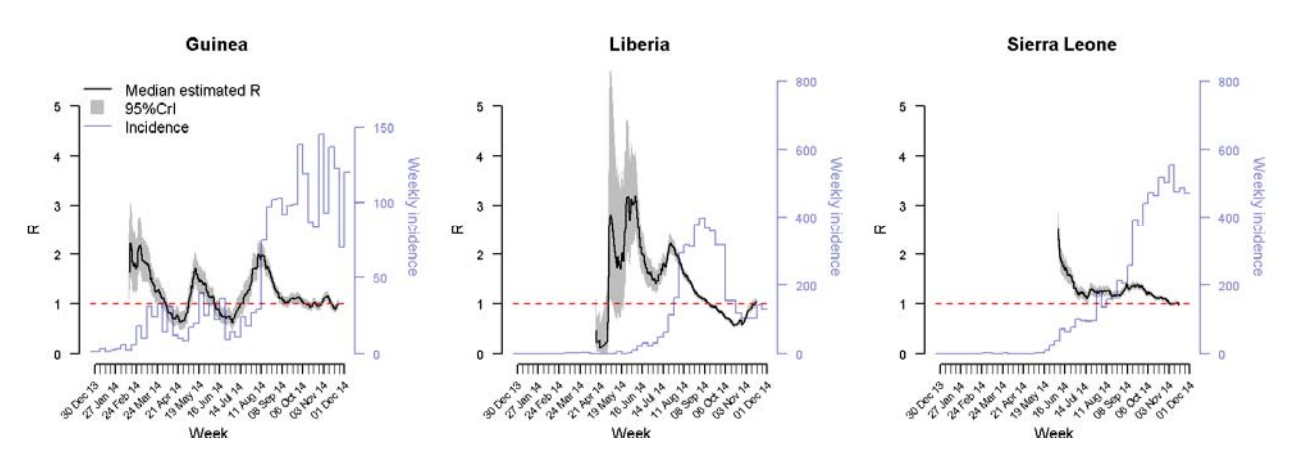
\includegraphics[width=\textwidth]{figures/WHO2}
		\caption{\textbf{[From \citep{WHO2015NEJM} (supplement), reproduced \emph{without} permission]}
	Shown are the estimated case reproduction numbers in Guinea, Liberia and Sierra Leone on the basis of data reported through December 7, 2014 for Guinea and November 30, 2014 in Liberia and Sierra Leone. $R_e$ was estimated over sliding 4-week windows and plotted at the midpoint of these windows.} 
		\label{fig:WHO}
	\end{figure}


\subsubsection*{Other parameters}

	Trends in sampling proportion estimates follow empirical estimates based on the number of confirmed cases, however the sampling proportion is overestimated during the period of intense transmission, which suggests unsampled transmission chains not represented in the dataset. 
	In the final two months of the study period the sampling proportion is underestimated, which may indicate ongoing cryptic transmission during this period, but may also be indicative of a model bias resulting from the remaining transmission chains at this time being highly isolated from each other, which is not taken into account by the model. 

	The estimated origin time of the epidemic coincides with the onset of symptoms and the death of the suspected index case \citep{WHO2016NEJM} on December 26 and 28, 2013, respectively (although earlier reports placed it at the start of December 2013 \citep{Baize2014NEJM}). 

	The median tMRCA estimate is February 16, 2014 (95\% HPD interval Jan 22--March 3, 2014), which overlaps with estimates reported in \citet{Dudas2017Nature} using all 1,610 sequences (95\% HPD interval December 16, 2013--February 20, 2014).

	The median estimate for the infected period, time from being infected to losing infectiousness (\ie incubation + infectious periods) is 13 days (95\% HPD interval 11.15--15.21 days). This period includes the incubation and infectious periods. This time period should roughly correspond to the generation time (when assuming that most infected patients do not cause multiple secondary infections, which agrees with $R_e < 2$), the time from infection of an index case to infection in a secondary infection. The generation time is difficult to estimate, but follows the same distribution as the serial interval, the time interval between symptom onset in an index case and symptom onset in a secondary case \citep{WHO2014NEJM}. 
	WHO estimates of the serial interval is 13 days (IQR 8--18 days) \citep{WHO2015NEJM}, which agrees with the bdsky estimates for the infected period.

	The median posterior estimate of the mean clock rate was $1.01 \times 10^{-3}$ s/s/y (95\% HPD interval $0.9-1.08 \times 10^{-3}$ s/s/y). This is slightly slower than estimates using the complete dataset of 1,610 sequences and the coding and noncoding regions of the genome. \citet{Holmes2016Nature} reported a median estimate of $1.2 \times 10^{-3}$ s/s/y (95\% HPD interval $1.13-1.27 \times 10^{-3}$). This is to be expected, since there are more substitutions in the noncoding part of the genome, resulting in a faster clock rate when using both coding and noncoding regions.




	\clearpage
	\printbibliography


\end{document}












